% This is samplepaper.tex, a sample chapter demonstrating the
% LLNCS macro package for Springer Computer Science proceedings;
% Version 2.20 of 2017/10/04
%
\documentclass[runningheads]{llncs}
\usepackage[english]{babel}
% for in-text and parentheis citations (works with technopress bib style)
\usepackage[round, authoryear]{natbib}
% for hyperlinking cross-references
\usepackage{hyperref}
% For figures
\usepackage{graphicx}
% For block quotes (see https://tex.stackexchange.com/questions/325695/how-to-style-blockquote and https://tex.stackexchange.com/questions/140300/how-to-prevent-pagebreak-in-quote-environment)
\usepackage{etoolbox}
\usepackage{setspace} % for \onehalfspacing and \singlespacing macros
% For multiple images in one figure
\usepackage{subcaption}
% For curly math letters for vocabulary reuse graph
\usepackage{mathrsfs}
% For \text in equations
\usepackage{amsmath}

%% for multiple comma-separated footnotes (see https://tex.stackexchange.com/questions/40072/incompatibility-between-footmisc-option-multiple-and-hyperref/62091#62091)
%! suppress = DiscouragedUseOfDef
\let\oldFootnote\footnote
\newcommand\nextToken\relax
\renewcommand\footnote[1]{\oldFootnote{#1}\futurelet\nextToken\isFootnote}
\newcommand\isFootnote{\ifx\footnote\nextToken\textsuperscript{,}\fi}

% For block quotes
\newenvironment{nbquote} {\quote\interlinepenalty=10000 } {\endquote}
\AtBeginEnvironment{nbquote}{\par\singlespacing\footnotesize}

% Used for displaying a sample figure. If possible, figure files should
% be included in EPS format.
%
% If you use the hyperref package, please uncomment the following line
% to display URLs in blue roman font according to Springer's eBook style:
% \renewcommand\UrlFont{\color{blue}\rmfamily}

\begin{document}
%
    \title{CS 715 Seminar Thesis}
    \subtitle{Linked Data on the Web}
%
%\titlerunning{Abbreviated paper title}
% If the paper title is too long for the running head, you can set
% an abbreviated paper title here
%
    \author{Lukas M. Loos}
%
%\authorrunning{F. Author et al.}
% First names are abbreviated in the running head.
% If there are more than two authors, 'et al.' is used.
%
    \institute{University of Mannheim}
%
    \maketitle              % typeset the header of the contribution
%
    \begin{abstract}
        Linked open data (LOD) is data published on the web following certain technological standards that are supposed to facilitate the datasets' integration.
        LOD has been adopted very extensively in the domain of life sciences (LSLOD).
        In this area, the most prominent publishers are the projects Bio2RDF and BioPortal.
        The growth of LSLOD has decreased in the recent years and some projects, like Bio2RDF, have not been maintained for several years.
        Other projects, like BioPortal, however, are still being maintained actively.
        Since LOD was developed for data integration in the first place, its application mainly focuses on this purpose too.
        Some companies are already using it in production.
        However, currently, the technologies' application always with large amounts of manual effort.
        Limited accessibility and availability and semantic heterogeneity are challenges users have to face when working with LSLOD and make the datasets' integration harder than initially intended.
        For example, $78\%$ of the datasets in the LSLOD-cloud were not accessible via the provided metadata and while there is a large amount of term overlap between the datasets, overlapping terms are mostly described with unique identifiers, preventing their automatic integration.

    \end{abstract}


    \section{Available Data}

    \subsection{Linked Open Data}
    When \citet{berners2001semantic} introduced the idea of the semantic web as an evolution of the original document web, their vision was to allow agents to infer the meaning of instances and their relationships published in datasets on the web.
    This is enabled by assigning instances and relations to URIs from standardized vocabularies, making their meaning no more limited to the dataset's scope but globally valid.
    The semantic web relies on various technological standards of which some were specifically developed for it and others already existed.

    Firstly, just like the document web, it relies on HTTP for data transmission.
    RDF~\citep{RDF}, a standard published by the World Wide Web Consortium (W3C) is the recommended language for transferring linked data and describes datasets as collections of triples consisting of subjects, predicates, and objects.
    Vocabularies for linked data are organized in ontologies, defined in the standards RDFS~\citep{RDFS} and OWL~\citep{OWL}.
    Finally, SPARQL~\citep{SPARQL}, another standard by the W3C is a query language that can be used to query linked datasets.

    \subsection{Linked Open Data Cloud}
    Probably the most prominent service around linked open data is the Linked Open Data Cloud (LOD-cloud)
    \footnotemark{} (see Figure~\ref{fig:lod_cloud}).
    The LOD-cloud is a diagram visualizing linked open datasets and their interconnections.

    \begin{figure}[ht]
        \centering
        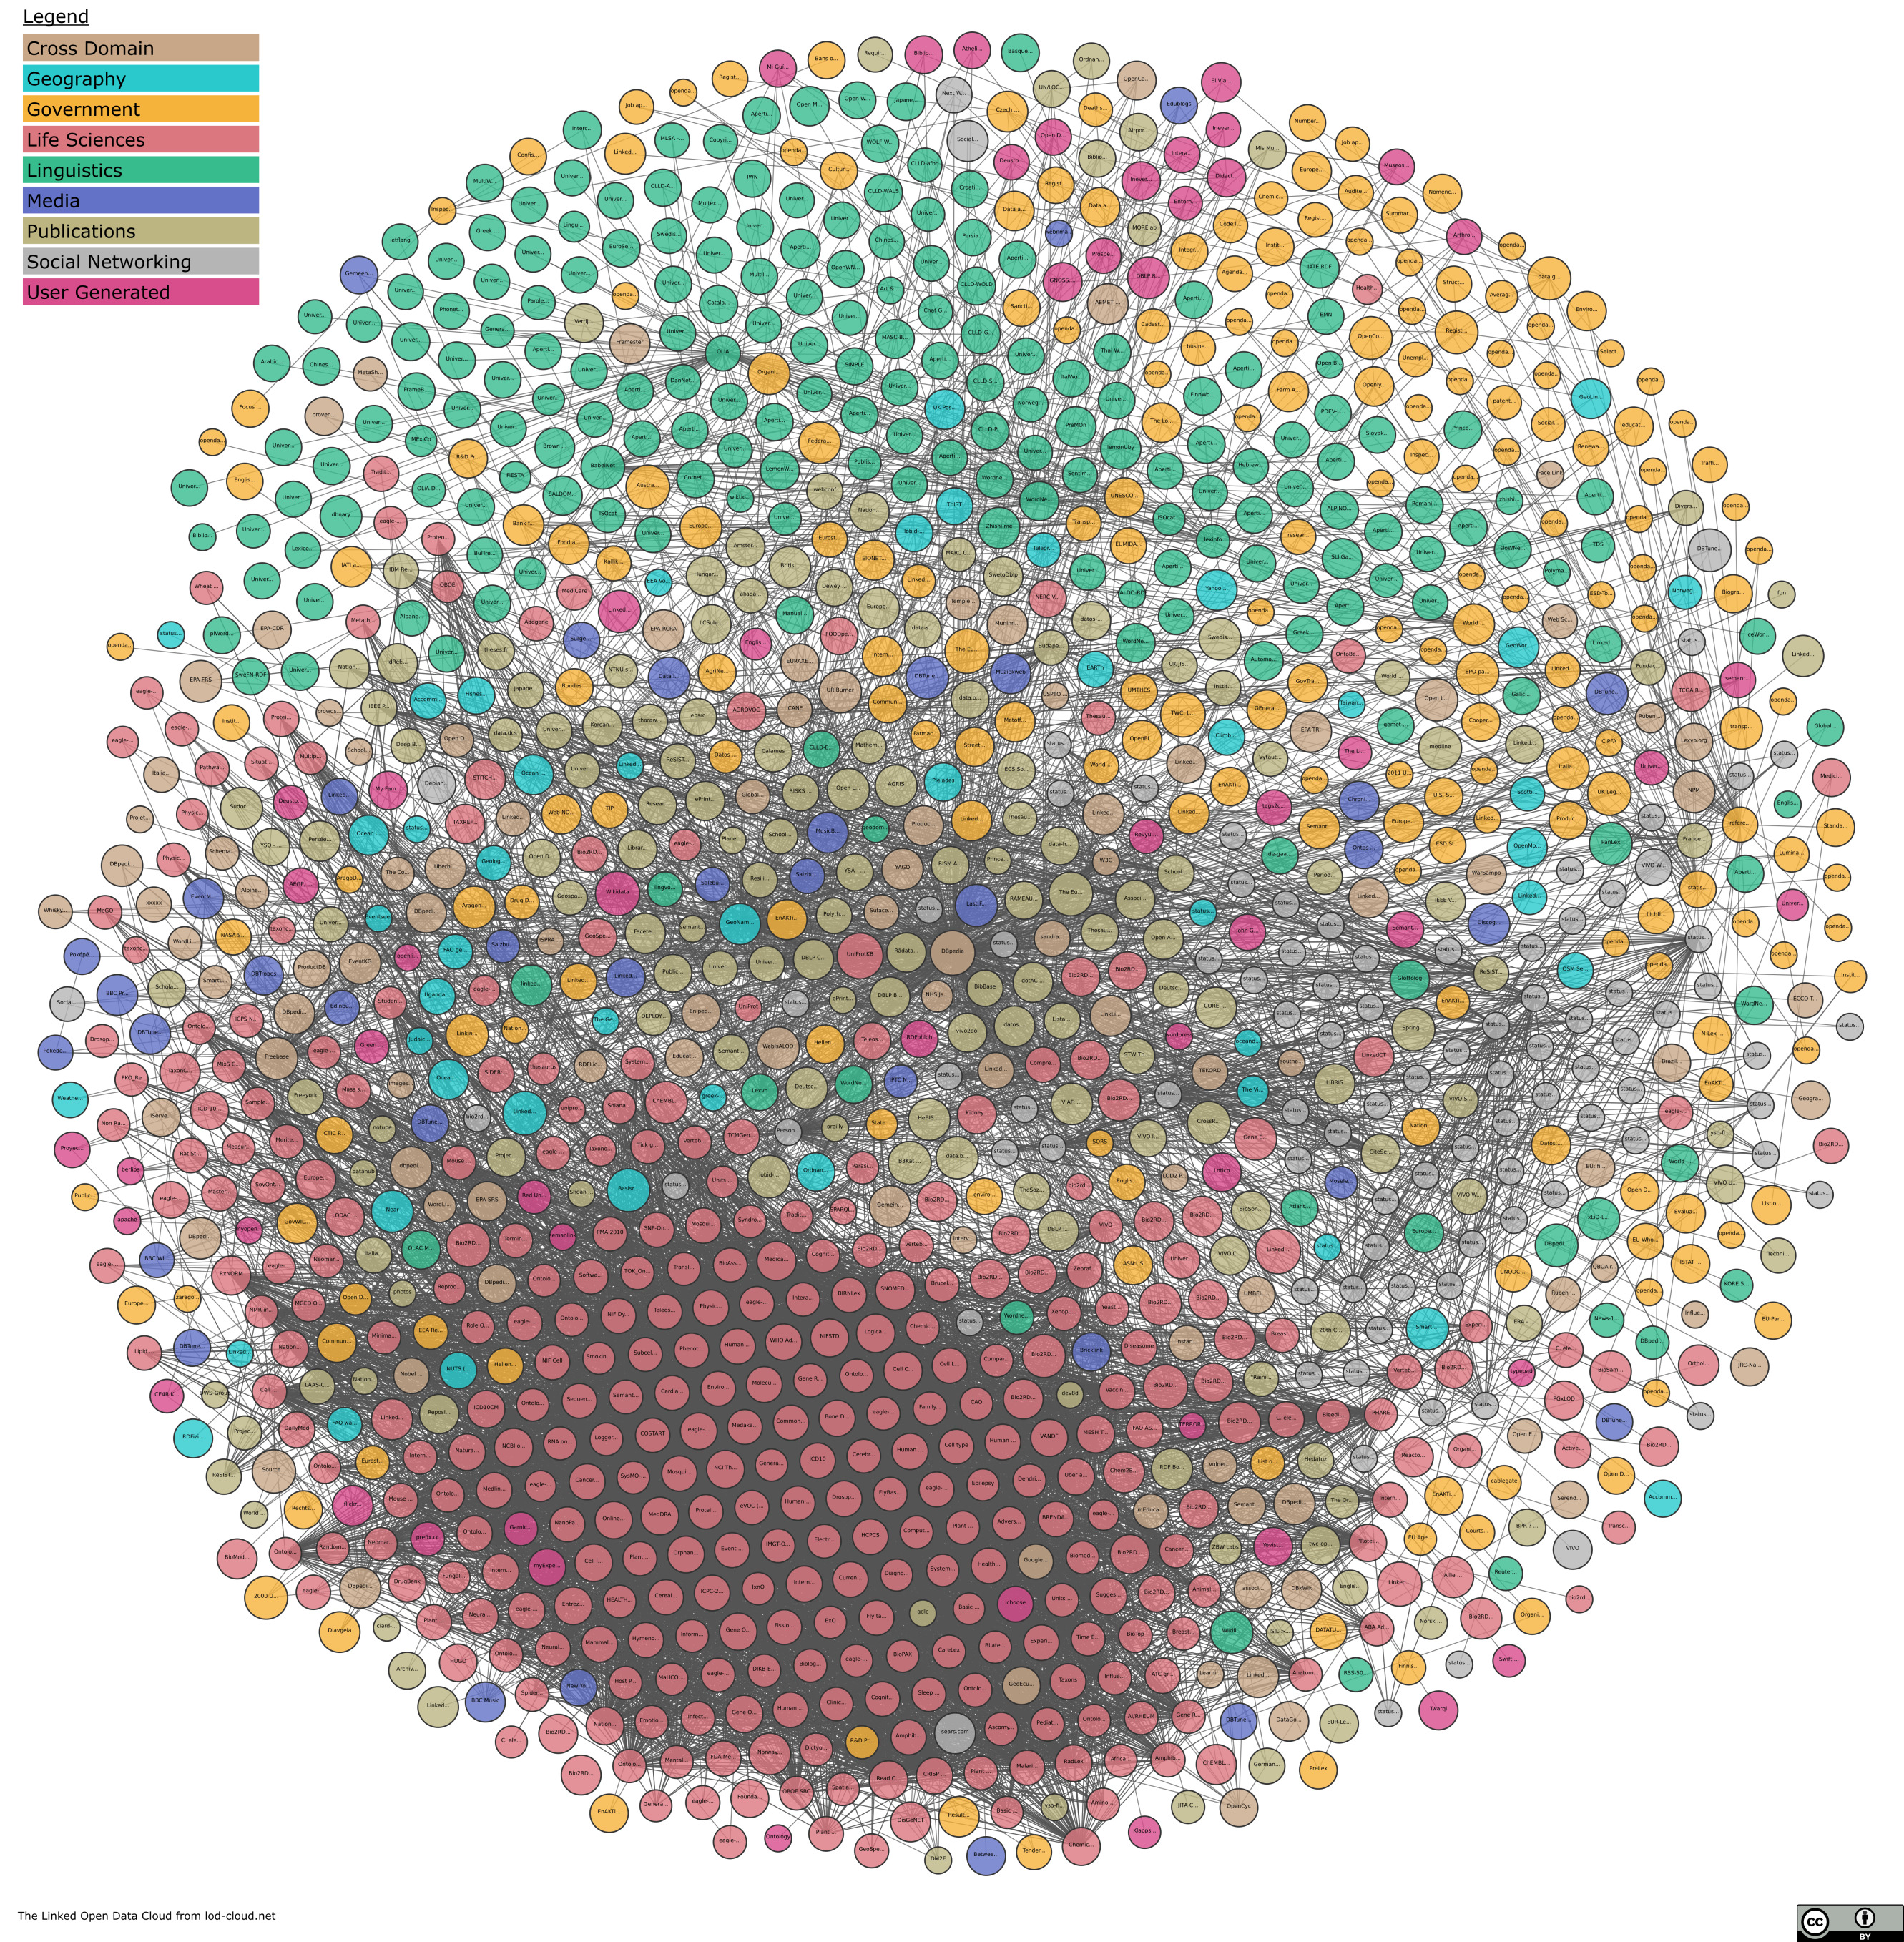
\includegraphics[width=\textwidth]{figures/lod-cloud-sm}
        \caption{The LOD-cloud\protect\footnotemark[\value{footnote}]}
        \label{fig:lod_cloud}
    \end{figure}

    For a dataset to be included, it has to meet certain requirements.
    For example, instances have to be annotated with URIs that resolve to RDF data, the dataset must contain at least 1000 triples, and it has to be connected via RDF links to datasets in the diagram with at least 50 links.
    The LOD-cloud also provides metadata about the datasets.
    For example, it divides the datasets into different domains, like Media, Government, Publications, Social Networking, or Life Sciences.
    As of May 2021 this catalogue contained 1301 datasets and has become the subject of multiple investigations~\citep{debattista2019lod, kamdar2019enabling, schmachtenberg2014adoption}.

    \subsection{Life Sciences Linked Open Data Cloud}
    In this thesis, I will focus on datasets from the life sciences domain, colored red in Figure~\ref{fig:lod_cloud}.
    This part of the LOD-cloud is often also referred to as life-sciences LOD-cloud (LSLOD-cloud) and is depicted in more detail in Figure~\ref{fig:lslod_cloud}.

    \begin{figure}[ht]
        \centering
        \includegraphics[width=\textwidth]{figures/life-sciences-lod}
        \caption{The LSLOD-cloud\protect\footnotemark[\value{footnote}]}
        \label{fig:lslod_cloud}
    \end{figure}
    \footnotetext{The Linked Open Data Cloud, https://lod-cloud.net/, (Accessed on 01/06/2022)}

    Biomedical researchers have already been adopting semantic web technologies in their early stages~\citep{ashburner2000gene, bodenreider2004unified, wang2005xml}, motivated by a problem that still exists in the domain and was addressed by Vijay Bulusu, head of data and digital innovation at company Pfizer:
    \begin{nbquote}
        Vijay Bulusu opened his plenary session at the Bio-IT World Conference \& Expo last week by asking the audience whether - if given \$1 million to spend - they'd buy a machine learning platform or improve the quality of their data.
        Nearly everyone voted for improving data quality.
        Bulusu was pleased.
        Life sciences doesn't really have a big data problem, he explained.
        It has a "lots-of-small-data problem," and data should be our focus~\citep{Pfizer}.
    \end{nbquote}
    Datasets in the LSLOD-cloud describe entities such as molecules (e.g., drugs or proteins) and their characteristics, biological pathways, organs, or diseases~\citep{bodenreider2008biomedical}.
    In their attempt to implement a query engine that was supposed to make SPARQL endpoints of LSLOD datasets more accessible, \citet{kamdar2014roadmap} catalogued linked concepts and properties from 137 public SPARQL endpoints to map concepts and properties to so-called Query Elements.
    Figure~\ref{fig:lslod_entities} gives an overview of the number of entities from the datasets linked to different types of Query Elements.

    \begin{figure}[ht]
        \centering
        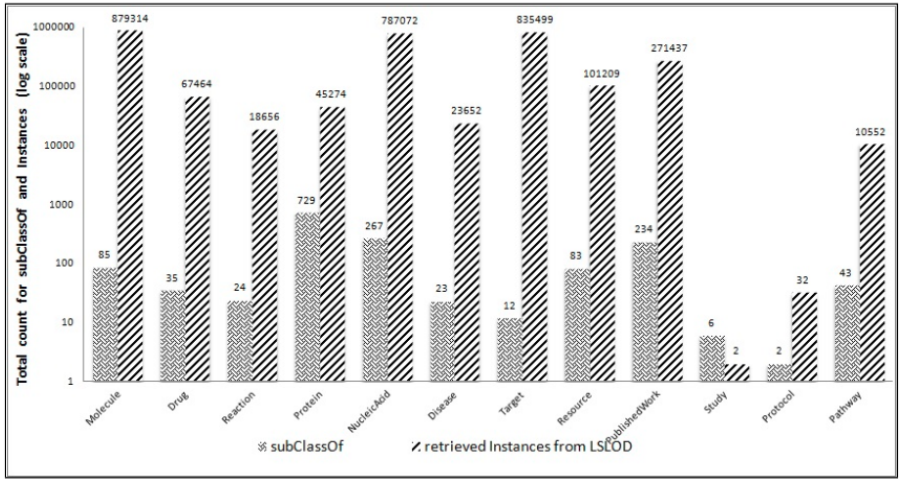
\includegraphics[width=\textwidth]{figures/lslod_entities}
        \caption{Representation of different types of entities in LSLOD Dataset~\citep{kamdar2014roadmap}.}
        \label{fig:lslod_entities}
    \end{figure}
    \footnotetext{The Linked Open Data Cloud, \url{https://lod-cloud.net/}, (Accessed on 01/06/2022)}

    \section{Data Publishers}
    A very large part of the datasets in the LSLOD-cloud are published two projects:
    NCBO BioPortal~\citep{BioPortal}, colored orange in the LSLOD-cloud, and Bio2RDF~\citep{Bio2RDF}, colored purple in the LSLOD-cloud.

    \subsection{BioPortal}
    BioPortal is a project funded by the National Institute of Health (NIH) and provides centralized access to a collection of biomedical ontologies.
    Since the provided datasets are ontologies, they do not contain any instance data, but define classes and properties that can be used as vocabularies to type instances in other datasets.
    In January 2022, the collection consisted of 953 ontologies, containing $13,732,155$ classes, and $36,286$ properties\footnote{NCBO BioPortal, \url{https://bioportal.bioontology.org/}, (Accessed on 01/08/2022)}.
    Only a subset of these ontologies are registered in the LSLOD-cloud.
    BioPortal is not the original publisher of the provided ontologies, but rather provide unified access to ontologies from different sources like SNOMED CT\footnote{SNOMED International, \url{https://www.snomed.org/}, (Accessed on 01/08/2022)}, a large, general purpose clinical ontology or RxNORM\footnote{RxNorm, \url{https://www.nlm.nih.gov/research/umls/rxnorm/index.html}, (Accessed on 01/08/2022)}, an ontology about clinical drugs which is part of the UMLS, another project related to the NIH that also provides linked data, however not using semantic web technologies.

    \subsection{Bio2RDF}
    Bio2RDF is an open source project maintained by Maastricht University and Universit\'e Laval and claims to provide the largest network of linked data in the domain of life sciences\citep{Bio2RDF_Github}.
    Like BioPortal, Bio2RDF are not the authors of the datasets they publish, but rather translated datasets from sources such as DrugBank\footnote{DrugBank Online, \url{https://go.drugbank.com/}, (Accessed on 01/08/2022)} or FarmGKB\footnote{PharmGKB, \url{https://www.pharmgkb.org/}, (Accessed on 01/08/2022)} into RDF\@.
    In contrast to BioPortal however, Bio2RDF provides LSLOD datasets with instance data and not ontologies.

    \subsection{Other LSLOD Publishers}
    An example for a publisher of LSLOD who is also the author of the provided datasets is the RDF Platform of the European Bioinformatics Institute (EBI)\footnote{RDF Platform, \url{https://www.ebi.ac.uk/rdf/}, (Accessed on 01/09/2022)}.
    The EBI is part of the European Molecular Biology Laboratory (EMBL), a research organization, funded by the governments of its 27 member states and provides SPARQL access points to several databases with biomedical data.

    Pharmaceutical companies, certainly among the main players in the biomedical domain have a seemingly conflicting relation to linked open data.
    I researched the practices of data sharing of the 3 largest companies by market capitalization\footnote{Largest pharma companies by market cap, \url{https://companiesmarketcap.com/pharmaceuticals/largest-pharmaceutical-companies-by-market-cap/}, (Accessed on 01/09/2022)}, namely, Johnson \& Johnson, Roche and Pfizer.
    On the one hand, these companies are in possession of large amounts of data of immense public value, and while they do claim to share data from clinical trials over various channels\footnote{Roche - Our commitment to data sharing, \url{https://www.roche.com/research_and_development/who_we_are_how_we_work/research_and_clinical_trials/our_commitment_to_data_sharing.htm}, (Accessed on 01/09/2022)}\footnote{Advancing Clinical Trial Data Sharing Through the Yale University Open Data Access Project | Johnson \& Johnson, \url{https://www.jnj.com/innovation/yale-open-data-access-project}, (Accessed on 01/09/2022)}\footnote{Data Access Requests | Pfizer, \url{https://www.pfizer.com/science/clinical-trials/trial-data-and-results/data-requests}, (Accessed on 01/09/2022)}, none of them seem to do so via linked open data.
    On the other hand, the companies seem to be aware of the potential value of the technologies.
    For example, representatives of Johnson \& Johnson and AstraZeneca have taken part in the W3C Linking Open Drug Data project~\citep{jentzsch2009linking, marshall2012emerging}.
    Some companies even seem to be using the technologies and public datasets already internally.
    For example, Pfizer's IDF Data Cloud, a project that is still in development, uses semantic web technologies to integrate LSLOD from various sources~\citep{Pfizer}.

    \section{Change of LSLOD over the Last Years}
    \subsection{Datasets in the LOD-cloud}
    \citet{schmachtenberg2014adoption} compared the adoption of LOD best practices in LOD-cloud datasets in 2011 and 2014.
    I augmented their data with LOD-cloud metadata from the years 2018--2021, retrieved from archive.org\footnote{Internet Archive: Wayback Machine, \url{https://archive.org/web/}, (Accessed on 01/09/2022)}.
    Figure~\ref{fig:lod-cloud-change} shows the change in the number of datasets in different domains over the recent years.
    While especially in the life-sciences domain, the number has been increasing relatively fast until 2018, this trend seems to have slowed down in the recent years.
    This trend seems not to exclusively affect the domain of life-sciences.
    The domain of linguistics seems to show a similar trend and other domains' growth (e.g., publications) has stopped already much earlier.

    \begin{figure}[ht]
        \centering
        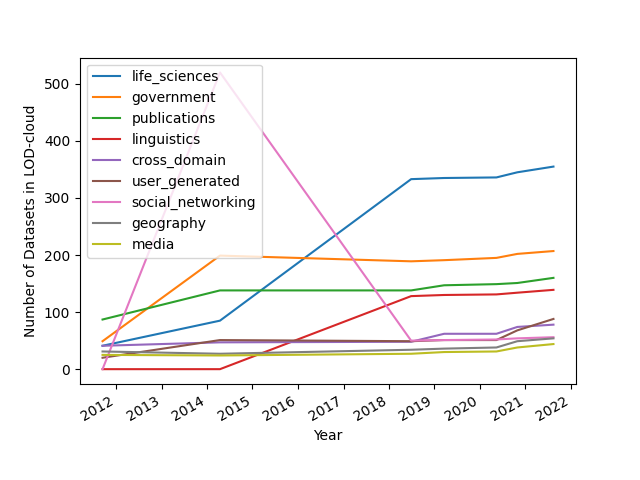
\includegraphics[width=0.7\textwidth]{figures/lod-cloud-change}
        \caption{Change in the number of datasets in the LOD-cloud over the recent years by domain.}
        \label{fig:lod-cloud-change}
    \end{figure}

    \subsection{Maintenance}
    Another aspect of LSLOD currency is whether the datasets are being actively maintained.
    Figure~\ref{fig:bioportal-maintenance} illustrates the time that has passed since the last time that ontologies in BioPortal have been updated.
    There are some ontologies that haven't been updated in several years, but overall it shows that much more both small and large ontologies have seen an update in the last year.

    \begin{figure}[ht]
        \centering
        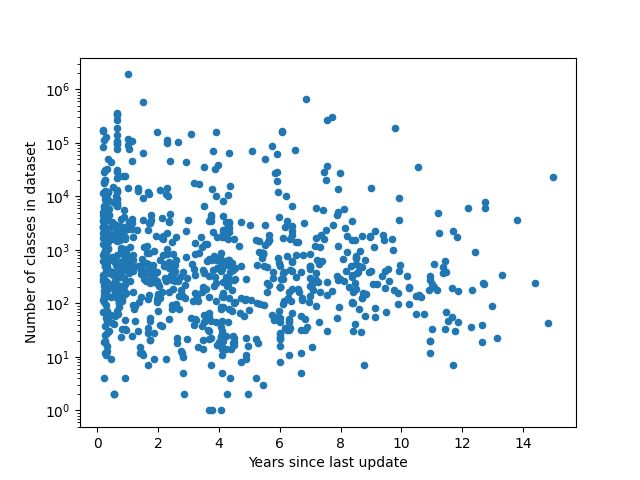
\includegraphics[width=0.8\textwidth]{figures/bio-portal-maintenance}
        \caption{Years since last update of datasets in BioPortal by number of classes in each dataset.}
        \label{fig:bioportal-maintenance}
    \end{figure}

    Unfortunately, it's different for the datasets provided by Bio2RDF and the EBI RDF Platform.
    Bio2RDF was last updated in 2014~\citep{Bio2RDF_Github} and the EBI RDF Platform has seen its last update in 2017 and states on its webpage that the project has run out of funding\footnote{New RDF platform released!, \url{https://www.ebi.ac.uk/rdf//2017/07/10/first-post/}, (Accessed on 01/09/2022)}.


    \section{Applications using LSLOD}
    The technologies behind LOD were initially introduced to tackle the challenge of integrating the ever-growing mass off datasets available on the web.
    As mentioned before, this challenge is particularly present in the domain of Life Sciences.
    As a consequence, there have been numerous research projects that have employed semantic web technologies to integrate LSLOD\@.

    For example, the W3C Linking Open Drug Data Project mentioned earlier, and a web data integration platform introduced by \citet{williams2012open} aim at integrating drug-related data~\citep{jentzsch2009linking}.
    \citet{saleem2014big} and \citet{sioutos2007nci} ran research projects investigating the integration of cancer-related datasets and \citet{kamdar2019enabling} investigated web-scale data integration with LOD in general in the areas of pharmacology, cancer research, and infectious diseases.
    An alternative approach was taken by \citet{percha2018global} who deployed an NER-based annotator and dependency parsing to automatically extract linked data from medline abstracts and compared the results to manually curated databases of linked data.

    On the other hand, the technologies have also already been adopted by several companies, using subsets of the LOD datasets in biomedical applications.
    Not only Pfizer is using LSLOD datasets in their IDF Data Cloud~\citep{Pfizer}.
    For example, Google is using LSLOD sources to augment their knowledge graph:
    \begin{nbquote}
        We worked with a team of medical doctors (led by our own Dr. Kapil Parakh, M.D., MPH, Ph.D.) to carefully compile, curate, and review this information.
        All of the gathered facts represent real-life clinical knowledge from these doctors and high-quality medical sources across the web, and the information has been checked by medical doctors at Google and the Mayo Clinic for accuracy~\citep{Aremedyf53:online}.
    \end{nbquote}
    IBM trained their supercomputer Watson on LSLOD datasets to assist with decision-making in oncology~\citep{doyle2015watson} and NuMedii, a biotechnology in San Mateo, California, uses semantic web technologies for drug research by integrating multiple public and private datasets~\cite{dastgheib2018accelerating}.
    Finally, there is an annotator tool for biomedical texts that is based on LSLOD and was developed by \citet{kamdar2020text}.


    \section{Integrability of LSLOD}
    As mentioned before, the primary goal of developing semantic web technologies was to make data more easily integrable.
    However, even though the technologies have already been deployed in various research problems, their use is almost always connected to a substantial amount of manual effort.

    This problem has motivated various authors to investigate its cause.
    \citet{heath2011linked} introduced a set of seven best practices that are required for LOD to be usable as originally intended.
    These best practices include measures of making the data accessible, like providing dereferenceable URIs and listing additional access methods, measures of guaranteeing integrability of the provided data, like linking the dataset to other datasets and using public vocabularies, and measures of increasing the usability of the data by providing relevant metadata.

    The adoption of these practices and extensions thereof have been investigated by multiple studies~\citep{schmachtenberg2014adoption, debattista2018evaluating, debattista2019lod}
    \citet{kamdar2019enabling} identified three major challenges for using LSLOD in applications, that partly reflect a lack of fulfillment of these principles: accessibility and availability, semantic heterogeneity, and learnability and usability.

    \subsection{Accessibility and Availability}
    Accessibility and availability of LOD sources in terms of dereferenceability of proprietary vocabularies has been investigated by \citet{schmachtenberg2014adoption}.
    They found that only about 28\% of proprietary vocabularies used in LSLOD datasets were actually dereferenceable.
    6\% of the vocabularies were only partially, and 67\% were not dereferenceable at all.
    \citet{debattista2019lod} investigated accessibility of LOD datasets by testing the availability of datasets via the methods provided in the LOD-cloud's metadata.
    I repeated this experiment, limiting the selection to datasets from the life sciences domain.
    Figure~\ref{fig:accessibility} shows the results of both experiments.
    According to Figure~\ref{fig:accessibility-2019}, in 2019, 66.8\% of the LOD datasets were not accessible at all.
    In 2021, I found for LSLOD datasets, that none of them was accessible by just using the SPARQL endpoint metadata provided in the metadata and also none was accessible via more than 1 method.
    In general 78\% of the datasets listed in the LSLOD cloud were not accessible by any of the methods described in the LOD cloud metadata.

    \begin{figure}[ht]
        \begin{subfigure}{0.545\textwidth}
            \centering
            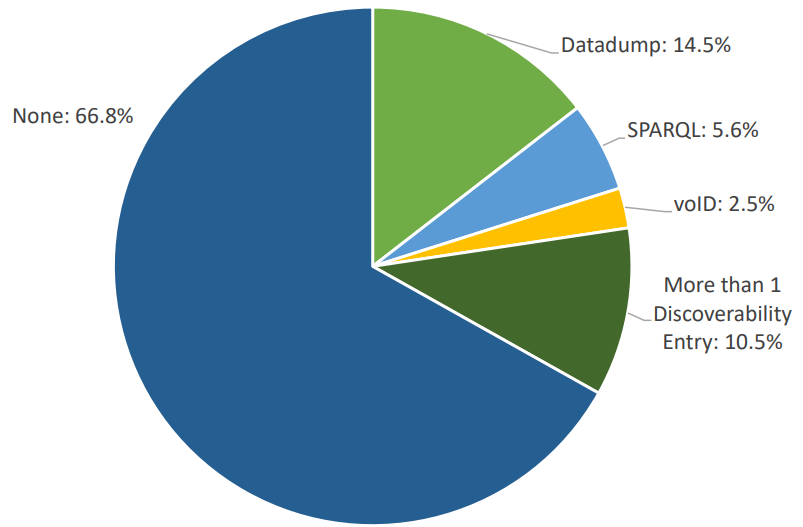
\includegraphics[width=\linewidth]{figures/accessibility-2019}
            \caption{Accessibility of LOD datasets~\citep{debattista2019lod}}
            \label{fig:accessibility-2019}
        \end{subfigure}
        \begin{subfigure}{0.455\textwidth}
            \centering
            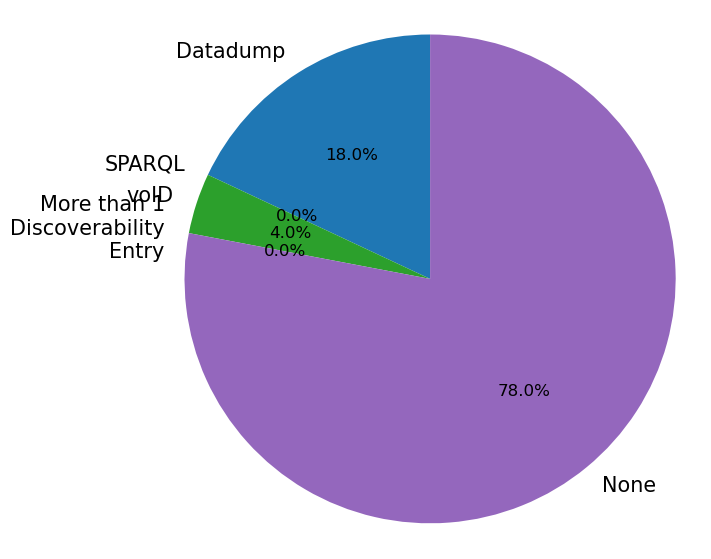
\includegraphics[width=\linewidth]{figures/accessibility-2021}
            \caption{Accessibility of LSLOD datasets in 2021}
            \label{fig:accessibility-2021}
        \end{subfigure}
        \caption{Results of experiments investigating accessibility of LOD datasets via methods described in LOD-cloud metadata}
        \label{fig:accessibility}
    \end{figure}

    \subsection{Semantic Heterogeneity}
    \citet{kamdar2021empirical} refer to semantic heterogeneity as the degree to which LSLOD sources use heterogeneous schemas, lack mappings between similar entities, and use different vocabularies for the same topics.
    However, another important factor is whether existing reuse or mappings are actually correct.
    The following paragraphs will look into these two aspects of semantic heterogeneity.

    \paragraph{Vocabulary Reuse}
    \citet{kamdar2017systematic} compared term reuse and term overlap in biomedical ontologies published by BioPortal.
    They defined term reuse as either the reuse of identical URIs or the existence of explicit mappings via either properties such as \texttt{owl:sameAs} or \texttt{owl:equivalentClass} (CUI), or explicit reference (xref).
    They defined term overlap as a cosine similarity of more than $.95$ between count vectors of instance labels enriched with varying sources such as synonyms, label annotations, or comments.
    To compute a statistic for term reuse/overlap across the ontologies, they first computed a graph $\mathscr{M}_{r}$ where each term in each ontology is represented as one of the $N$ nodes and reuse/overlap of terms according to the various definitions is represented as an edge between nodes.
    The resulting graph consisted of connected components of which the authors denoted those $k$ components with more than one term as $T_j$.
    The number of terms in component $T_j$ is denoted by $n_j$.
    Term reuse/overlap was then computed via Formula~\ref{eq:reuse}:
    \begin{equation}\label{eq:reuse}
        \text{Reuse/Overlap}=\frac{\sum_{j \mid T_{j} \in \mathscr{M}_{r}} n_{j}-k}{N}
    \end{equation}

    While the authors found a term overlap of approximately $25 - 31\%$, depending on the enrichment scheme, the term reuse only amounted to $5.98 - 8.39\%$, depending on the types of mappings considered.
    Furthermore, they report that most ontologies reuse only less than $5\%$ of their vocabulary.

    \citet{kamdar2021empirical} investigated vocabulary reuse in LSLOD sources with instance data, such as the datasets provided by Bio2RDF, that either had a functional SPARQL endpoint or were available as RDF data dumps and could be stored in a local SPARQL repository, and had at least 1000 instances under any classification scheme that could be queried through the SPARQL endpoint.

    As \citet{kamdar2017systematic}, they computed the reuse statistic with Formula~\ref{eq:reuse}, resulting in a vocabulary reuse of 19.86\%.
    However, the authors note that this high percentage is biased by the reuse of 30,251 ChEBI classes in only 4 sources.
    Instead of computing a term overlap statistic, they clustered the datasets into communities based on cosine similarity of 100-dimensional word embedding vectors generated from the instances' labels.
    Again, these communities suggested much more topical overlap than what is reflected in the vocabulary reuse.
    Besides that, they also revealed certain "identifier communities" that often contained different URI representations for similar entities.
    The authors called this phenomenon of incorrect mappings "intent for reuse".

    Figure~\ref{fig:vocabulary_reuse} illustrates reuse of the vocabularies that are used in the investigated datasets.
    The figure shows that most vocabularies are used by only very few sources.
    In fact, among those vocabularies that are used by more than 10 sources, only one vocabulary, the Gene Ontology, actually contains semantically meaningful domain-specific classes.
    All other frequently reused vocabularies instead specify languages for providing metadata (e.g., DCTERMS, SIO-CHEMINF) or schemata (e.g., RDFS, OWL2).

    \begin{figure}[ht]
        \centering
        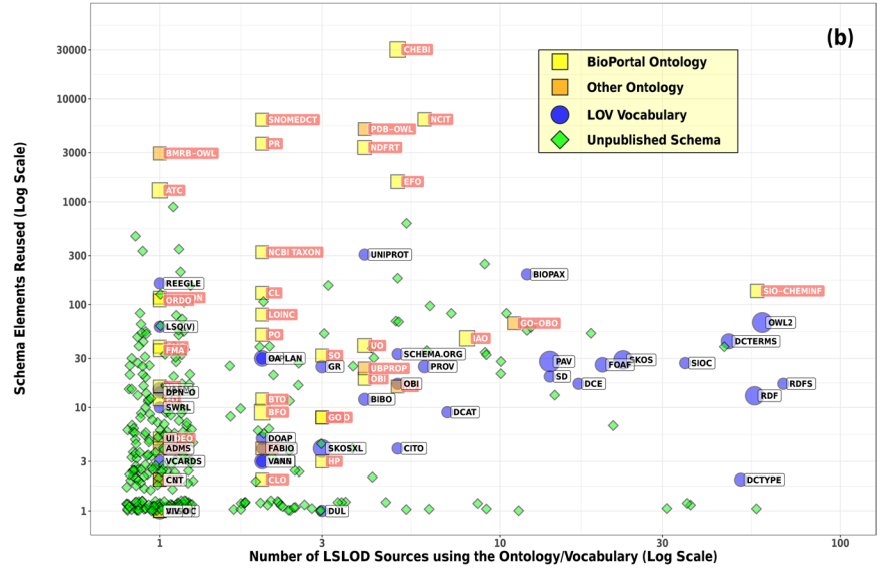
\includegraphics[width=\textwidth]{figures/vocabulary-reuse}
        \caption{Vocabularies used in LSLOD sources by number of sources using each vocabulary and number of elements from each vocabulary that are reused~\citep{kamdar2021empirical}.}
        \label{fig:vocabulary_reuse}
    \end{figure}

    Figure~\ref{fig:lslod-cloud-corrected} illustrates the interlinkage of lslod sources via vocabulary resource.
    According to the authors, this illustration can be perceived similar to the LSLOD cloud diagram depicted in Figure~\ref{fig:lslod_cloud} and shows that the LSLOD is actually much less interconnected than the LSLOD cloud diagram suggests.
    The figure also shows how especially Bio2RDF and EBI sources are very well interlinked.
    This fact makes it even more regrettable that, as mentioned before, both projects currently seem to be abandoned.

    \begin{figure}[ht]
        \centering
        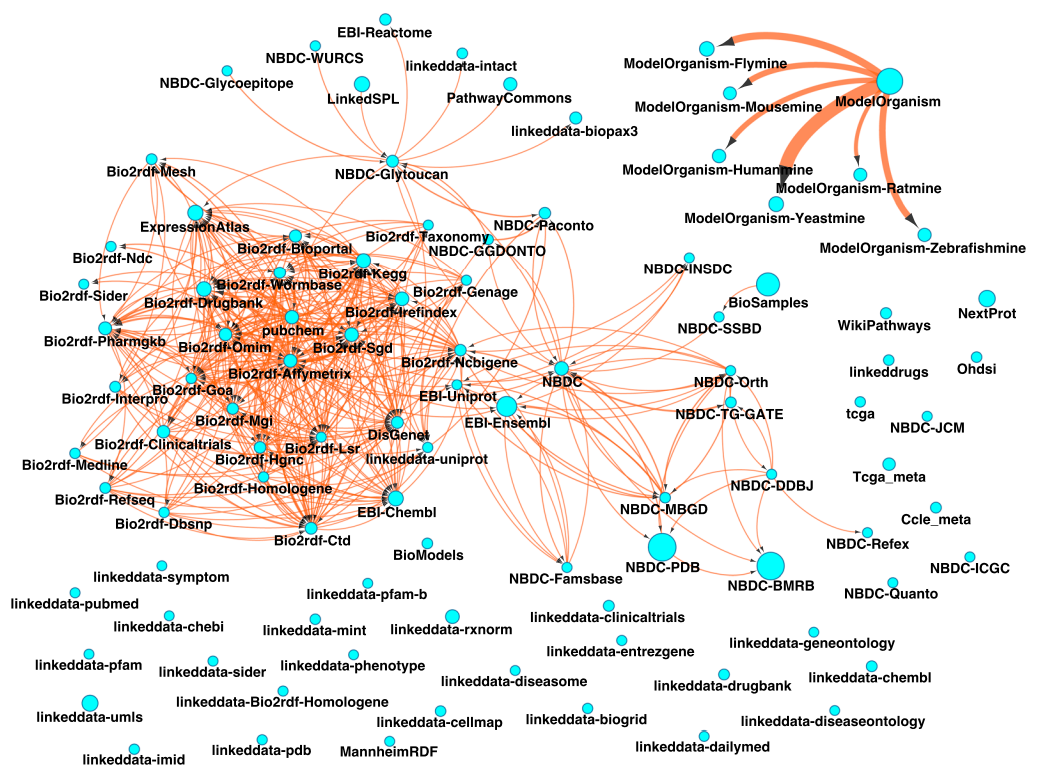
\includegraphics[width=\textwidth]{figures/lslod-connectedness}
        \caption{Vocabulary reuse among LSLOD sources. Each edge represents the existence of connections of entities between two LSLOD sources. The size of an edge represents the number of unique properties connecting entities in the two datasets~\citep{kamdar2021empirical}.}
        \label{fig:lslod-cloud-corrected}
    \end{figure}

    \subsection{Link Quality}
    Since I could not find any literature on the quality of mappings between LSLOD sources, I tried to verify the quality of the mappings in Bio2RDF and EBI datasets myself.
    For this purpose, I queried the SPARQL endpoints of Bio2RDF-Homologene Bio2RDF-Affymetrix, and EBI-Chembl with two different approaches.
    Unfortunately the EBI-Chembl SPARQL endpoint was not responsive at all, which may be related to the EBI RDF-Platform having run out of funding.
    For the remaining two datasets, I first investigated the use of \texttt{owl:sameAs} and \texttt{owl:equivalentClass}.
    The results indicated that the only mappings in the two datasets via these properties point to the domain \url{identifiers.org}, proving this method useless for investigating the mappings' quality.
    Second, I wrote SPARQL queries that were supposed to retrieve triples with objects from a different dataset by filtering the results via regular expressions so that only triples are retrieved whose object's URI starts with different domain name from the dataset's.
    However, this approach resulted in gateway-timeout errors, possibly because queries with regular expressions are very resource-intensive.

    \section{Conclusion}
    The stack of technologies behind linked open data was initially created to facilitate the integration of web data.
    However, the previous sections have shown that they are faced with substantial challenges that offer a rather bleak outlook at their application.
    The promise of effortlessly integrating data from different sources across the will certainly not be fulfillable in the near future.
    Nevertheless, there are also some promising movements in the semantic web community that are worth mentioning and show that still a lot of research is being conducted in this area.
    For example, \citet{verborgh2016triple} introduced Triple Pattern Fragments, which make maintaining SPARQL endpoints much less expensive and may contribute to solving the availability problem.
    Also, as described in the applications section, some companies with sufficient resources for curating the sources are already using some LSLOD datasets in production.
    Finally, in contrast to BioPortal and Bio2RDF, there are still very active LOD projects, like the earlier-mentioned Gene Ontology~\citep{gene2015gene} which has a strong community of domain users and a very active development team or DBPedia~\citep{auer2007dbpedia}, which according to \citet{kamdar2019enabling} have started registering $\approx99\%$ uptime, monitored via the SPARQLES framework~\citep{vandenbussche2017sparqles}.

%
% ---- Bibliography ----
%
% BibTeX users should specify bibliography style 'splncs04'.
% References will then be sorted and formatted in the correct style.
%
    \bibliographystyle{technopress}
    \bibliography{references}
%
\end{document}
